\chapter{Model Comparison}

In this section, we compare various model on the \emph{Pop} dataset. We start by describing a baseline model. We then implement a model from the literature and investigate its behaviour. We look at weighting the loss function, training on a more structured loss function, and performance of a transformer model. Finally, we investigate the use of generative features as input, experiment with decoding methods and compare the best models on the held-out test set.

\section{Logistic Baseline}

As a simple baseline, we consider a single layer NN which treats each frame independently. Then the layer takes input of size $216$ and outputs a $V$-dimensional vector, where $V$ is the cardinality of the chord vocabulary. The outputs are then passed through a softmax layer to get the probability of each chord and the cross-entropy loss is calculated. We call this model \emph{Logistic}.This can effectively be seen as a logistic regression model trained using stochastic gradient descent (SGD). We could have used a logistic regression model implemented in \texttt{sklearn} for example which may have found better minima but implementing it as a neural network was fast and easy and unlikely to yield significantly different results.

A grid search on learning rates and learning rate schedulers was conducted on the sets \texttt{[0.1, 0.01, 0.001, 0.0001]} and \texttt{[Cosine, Plateau, None]} respectively. The \texttt{Plateau} scheduler halves the learning rate when the validation loss hasn't improved for 10 epochs and \texttt{Cosine} is as described in Section~\ref{sec:training}. The best model was found to be a learning rate of $0.01$ with a \texttt{Cosine} scheduler. This best model was chosen for having the highest score on the most of the metrics in validation set. All models with learning rates of $0.01$ or $0.001$ converged within 150 epochs. Although the best model had learning rate $0.01$, a learning rate of $0.001$ over 150 epochs had a more stable validation accuracy. The model's results can be seen in Table~\ref{tab:baseline_results}. Full results are omitted as they are not relevant to the main discussion. The model serves simply as a baseline to compare the more complex models to. These results give us the first empirical evidence that the task is non-trivial. The model is only able to predict the root of the chord with a mean frame-wise accuracy of $0.64$ and a mirex of $0.65$. The model identifies both the root and the third with an accuracy of $0.56$ but struggles more with the seventh with an accuracy of $0.44$. The lowest scores are on class-wise accuracies able to predict the class of the chord with \texttt{class}\textsubscript{mean}$=0.13$ and \texttt{class}\textsubscript{median}$=0.03$. This gives us the first insight into each of the evaluation metrics and what we can hope from more complex models and other improvements.

\begin{table}[H]
    \centering
    \begin{tabular}{lcccccccc}
        \toprule
        Model & frame & root & third & seventh & mirex & class\textsubscript{mean} & class\textsubscript{median} \\  
        \midrule
        \emph{Logistic} & 0.42 & 0.64 & 0.56 & 0.44 & 0.65 & 0.13 & 0.03 \\
        \bottomrule
    \end{tabular}
    \caption{Baseline model results}\label{tab:baseline_results}
\end{table}

\section{CRNN}
\subsection{Model Description}

We implement a convolutional recurrent neural network (CRNN) as described in~\citet{StructuredTraining}. The model takes as input a matrix of size $I \times F$ where $I$ is the number of input features and $F$ is the number of frames. The model passes the input through a layer of batch normalisation, before being fed through two convolutional layers with ReLU after each one. The first convolutional layer has a $5\times 5$ kernel, and outputs only one channel the same size as the input. It is intended to smooth out noise and spread some information across adjacent frames about sustained notes. The second layer has a kernel of size $1\times I$, and outputs 36 values. This essentially acts as a linear layer across frames with shared inputs. The output is passed through a bi-directional GRU~\citep{GRU}, with hidden size initially set to $256$ and a final dense layer with the softmax activation. This produces a vector of length $V$ for each frame, where $V$ is the size of the chord vocabulary.

The authors of the model also propose using second GRU as a decoder before the final dense layer, called `CR2'. However, we believe that a similar effect could be achieved with more layers in the initial GRU. Furthermore, both in the paper and in brief empirical tests of our own, the results with `CR2' were indistinguishable from the model without it. We therefore do not include it in our final model. Results are omitted as they are neither relevant nor interesting.

\subsection{Small to Large Vocabulary}

Initial experiments were conducted on the simpler chord vocabulary with $V=25$. Only if the model could somewhat accurately classify the smaller vocabulary and if performance did not decrease on the smaller chord vocabulary when trained on the larger vocabulary, would we proceed to using the larger vocabulary. In keeping with with the methodology in~\citet{StructuredTraining}, we initially run with a learning rate of $0.001$. We reduce the learning rate to half its previous value if the validation loss hasn't improved in 10 epochs and stop training if it has not improved after 25 epochs, with a maximum of 100 epochs. Training samples were set to 10 seconds long. Model convergence was manually checked using the validation and training losses over epochs.

% A plot of the training history used to ensure check convergence is shown in Figure~\ref{fig:crnn_small_vocab_loss}.

% \begin{figure}[H]
%     \centering
%     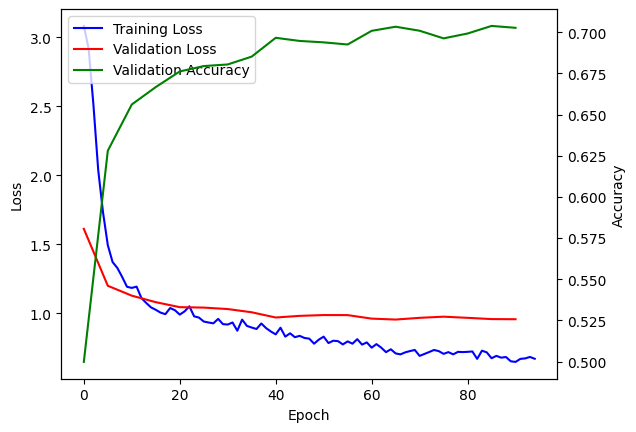
\includegraphics[width=0.8\textwidth]{figures/small_vocab_training_plot.png}
%     \caption{CRNN model training history on small vocabulary. We see the training loss and the validation loss and accuracy. The accuracy here is over all chord labels, not ignoring \texttt{X} as in final metric calculations. Training was stopped early at epoch 79. We can see the validation loss flattening out after around epoch 50. However, the model could have continued to be trained as it has not started overfitting yet. This behaviour later contributed to the argument for the removal of early stopping.}\label{fig:crnn_small_vocab_loss}
% \end{figure}

Results are shown in Table~\ref{tab:crnn_small_vocab}. For comparison, the table also shows the performance of the same model trained with the large vocabulary, $V=170$ and its predictions mapped back to the smaller vocabulary. A confusion matrix over chord roots of the model trained on $V=26$ is shown in Figure~\ref{fig:crnn_small_vocab_cm}. The model performs better than the baseline on the larger vocabulary, which is to be expected given the nested nature of the models, and the harder task on the larger vocabulary. From the confusion matrix, it becomes clear that many of the mistakes the model is making lie in the \texttt{X} symbol, which constitutes just over 7\% of the smaller vocabulary dataset. Chords with qualities like \texttt{sus4} could be confused with \texttt{major} by a reasonable model but are represented with \texttt{X} in the smaller vocabulary. Interestingly, the model trained with $V=170$ performs nearly as well on all metrics as the model trained with $V=25$. This implies that training with $V=170$ allows the model to learn almost all the relevant information about the smaller vocabulary, and gives it the chance to learn something about the larger vocabulary as well. Therefore, we proceed with the larger vocabulary for the rest of the experiments.

While some other works continue to measure performance on the smaller vocabulary~\citep{BTC}, we believe more metrics distract from the main goal of increasing performance across a wider range of chords. Additionally, the \texttt{third} metric capture much of the information we would look for in the evaluating with $V=25$. We therefore only measure performance on the larger vocabulary from now on.

\begin{table}[H]
    \centering
    \begin{tabular}{lcccccc}
        \toprule
        Model & $V$ for training & root & third & class\textsubscript{mean} & class\textsubscript{median} \\  
        \midrule
        \emph{CRNN} & 26 & 0.79 & 0.77 & 0.74 & 0.74 \\
        \emph{CRNN} & 170 & 0.78 & 0.74 & 0.72 & 0.73 \\
        \bottomrule
    \end{tabular}
    \caption{CRNN model results on the small vocabulary with $V=26$. The other metrics are omitted as they are identical to \texttt{third} for classification with $V=26$.}\label{tab:crnn_small_vocab}
\end{table}

\begin{figure}[H]
    \centering
    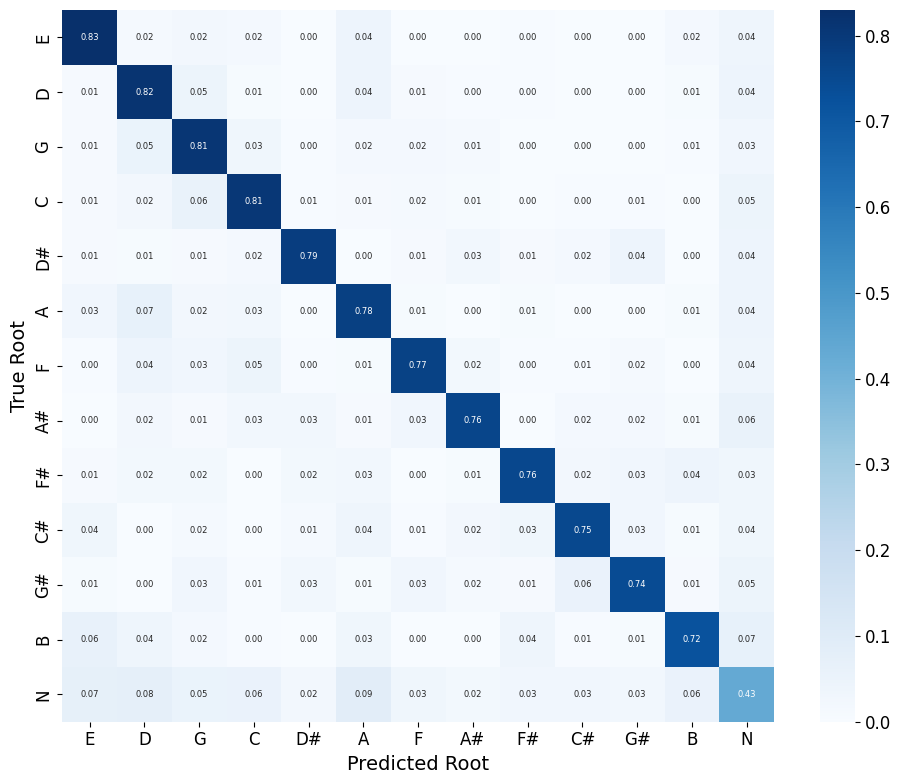
\includegraphics[width=1.0\textwidth]{figures/small_vocab_root_cm.png}
    \caption{Confusion matrix over roots of the CRNN model trained on the small vocabulary. The values have been normalised over rows such that the values on the diagonals are recall metrics. There is a clear outlier in the model's recall with the label \texttt{X}, at just $0.07$. It also performs poorly on \texttt{N}.}\label{fig:crnn_small_vocab_cm}
\end{figure}

\subsection{Hyperparameter Tuning}

After progressing to the larger vocabulary, we thought it a good time to conduct some hyperparameter tuning. 

\subsubsection{Learning rates}

We perform grid search on the same learning rates and learning rate schedulers as for the \emph{Logistic} model. The learning rates were in the set of \texttt{[0.1, 0.01, 0.001, 0.0001]} and the learning rate schedulers to \texttt{[Cosine, Plateau, None]}. We remove early stopping in order to check for convergence and overfitting without the possibility of a pre-emptive stop. Judging by training graphs seen in~\ref{fig:lr_search_cosine}, the best learning rate is $0.001$. Any lower and we do not converge fast enough; any higher and gradient updates cause the validation accuracy to be noisy. These figures also show that the validation loss does not get worse after convergence. We conclude that the model is not quick to overfit, perhaps due to the random sampling in the training process. Combined with the fact that training is relatively quick and we only save on improved validation loss, we decided to remove early stopping. We therefore conduct future experiments without early stopping and with \texttt{lr=0.001} and \texttt{Cosine} scheduling.

SGD has been shown to be a good optimiser for a longer run over many epochs if the model is able to converge [XX]. We ran an experiment over 2000 epochs with the above hyperparameters and \texttt{momentum=0.9} and found that the model was able to converge, reaching its best validation loss at around 1000 epochs and remaining flat thereafter. The results with this model did not improve on the best model trained with Adam, with 3\% lower root accuracy and 2\% lower third accuracy, but with 2\% better mirex. Due to the much longer training time and the lower root accuracy, we decided to stick with Adam for the rest of the experiments.

\begin{figure}[H]
    \centering
    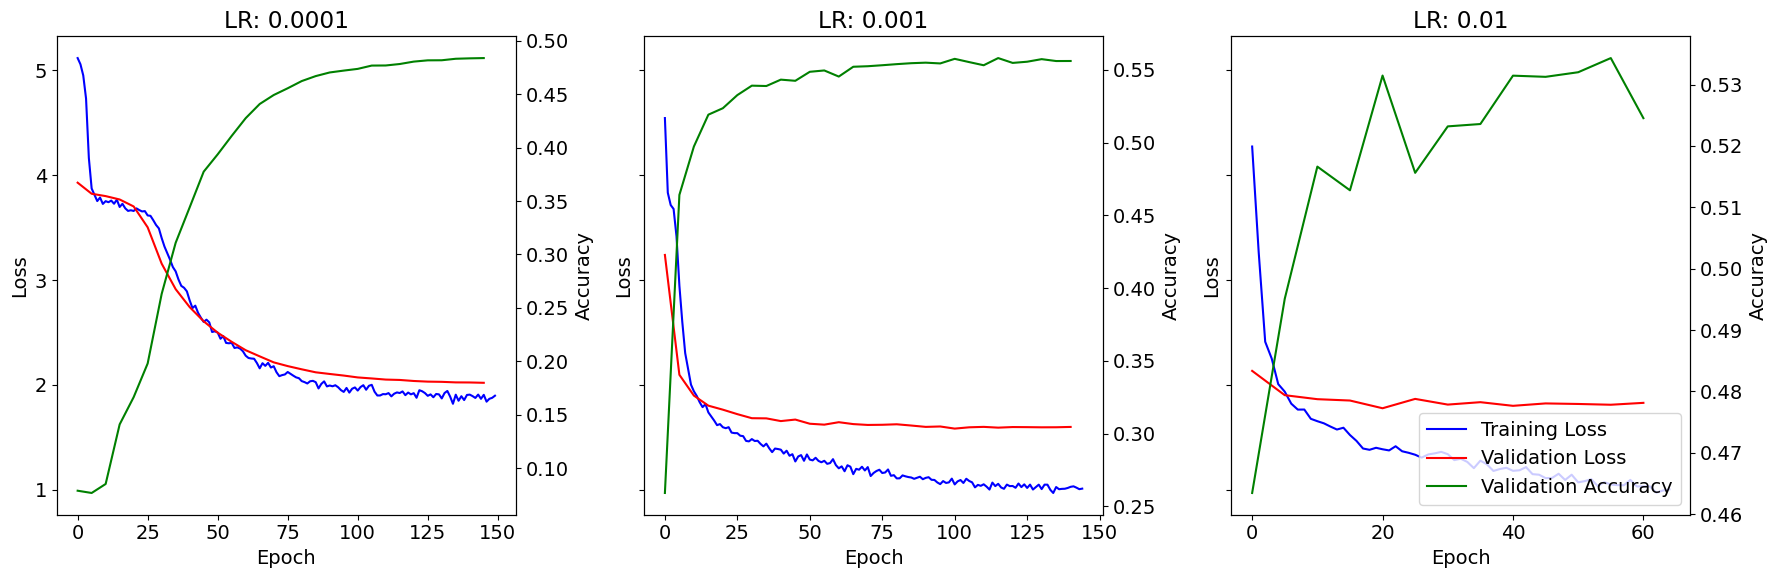
\includegraphics[width=1.0\textwidth]{figures/lr_search_cosine.png}
    \caption{Training graphs for the CRNN model with different learning rates. The learning rate of $0.001$ seems to be the best, as it converges in a reasonable time and the validation accuracy increases in a stable fashion.}\label{fig:lr_search_cosine}
\end{figure}

We report a subset of metrics in Table~\ref{tab:crnn_lr}. The best performing model by validation metrics was found to be with \texttt{lr=0.001} and \texttt{Cosine} scheduling. However, there were no large differences in performance between the learning rate schedulers. We proceed with these hyperparameters as defaults for the rest of the experiments.

\begin{table}[H]
    \centering
    \begin{tabular}{lccccccc}
        \toprule
        lr & scheduler & root & third & seventh & mirex & class\textsubscript{mean} & class\textsubscript{median} \\
        \midrule
        0.01 & Cosine & 0.71 & 0.68 & 0.55 & 0.76 & 0.13 & 0.00 \\
        0.001 & Cosine & \textbf{0.77} & \textbf{0.73} & \textbf{0.60} & 0.80 & 0.17 & \textbf{0.01} \\
        0.0001 & Cosine & 0.70 & 0.65 & 0.54 & 0.70 & 0.10 & 0.00 \\
        \midrule
        0.001 & Plateau & 0.74 & \textbf{0.73} & \textbf{0.60} & 0.80 & \textbf{0.18} & \textbf{0.01} \\
        0.001 & None & 0.71 & 0.70 & 0.58 & \textbf{0.82} & 0.17 & 0.00 \\
        \bottomrule
    \end{tabular}
    \caption{CRNN model results on the large vocabulary with different learning rates and schedulers. Overall, a learning rate of 0.001 and a scheduler of \texttt{Cosine} performs the best in many metrics, though a scheduler of \texttt{Plateau} performs just as well or better on many metrics. We prioritise the performance of the model on the root as this is more important than the \texttt{mirex} metric. }\label{tab:crnn_lr}
\end{table}

\subsubsection{Model Hyperparameters}

With this learning rate and learning rate scheduler fixed, we perform a random search on the number of layers in the GRU, the hidden size of the layers in the GRU and the training patch segment length. The search is performed by independently and uniformly randomly sampling 32 points in the sets $\texttt{hidden\_size}\in\{64,65,\ldots,512\}$, $\texttt{num\_layers}\in\{1,2,3\}$ and $\texttt{segment\_length}\in\{10,11,\ldots,60\}$. A sample of the results are shown in Table~\ref{tab:crnn_hparams}. The models were then ranked according to each metric and their ranks for each metric added up. The models were ordered by this total rank. The best model was found to have a hidden size $h=201$, a single layer GRU and a segment length of $L=28$, although the differences between models were relatively small. Such small differences might indicate that the model is learning something relatively simple and that increased model complexity will not help. We proceed with this model as the default for the rest of the experiments, referred to simply as the \emph{CRNN}.

\begin{table}[H]
    \centering
    \begin{tabular}{cccccccccc}
        \toprule
        $L$ & layers & $h$ & frame & root & third & seventh & mirex & class\textsubscript{mean} & class\textsubscript{median} \\
        \midrule
        28 & 1 & 201 & \textbf{0.58} & \textbf{0.78} & 0.75 & 0.62 & \textbf{0.79} & 0.18 & 0.01 \\
        23 & 2 & 295 & 0.58 & 0.78 & \textbf{0.75} & \textbf{0.62} & 0.78 & 0.19 & 0.02 \\
        14 & 2 & 374 & 0.57 & 0.77 & 0.74 & 0.61 & 0.79 & 0.19 & \textbf{0.02} \\
        56 & 1 & 463 & 0.58 & 0.77 & 0.74 & 0.61 & 0.78 & 0.19 & 0.02 \\
        42 & 3 & 222 & 0.57 & 0.77 & 0.74 & 0.60 & 0.79 & 0.16 & 0.00 \\
        \ldots & \ldots & \ldots & \ldots & \ldots & \ldots & \ldots & \ldots & \ldots \\
        \bottomrule
    \end{tabular}
    \caption{CRNN model results on the large vocabulary with different hyperparameters. Best unrounded metrics are bolded. Results across all hyperparameters were very similar. We proceed with the best model found with hidden size of $201$, a single layer GRU and a segment length of $28$, although any configuration would work similarly. This also implies that model is learning something simple because the increased complexity of larger models did not help with performance. The variance within the data may be entirely due to the stochastic nature of SGD. Regardless of what makes the results different, the effect size is small enough that we conclude it does not make a difference.}\label{tab:crnn_hparams}
\end{table}

Hyperparameters for CQT computation were chosen to be the same as in~\citet{StructuredTraining}. However, the hop length was chosen to be $4096$ samples. Other works have used 512 samples~\citet{ACRLargeVocab1} or $2048$ samples~\citet{CurriculumLearning}. It should be noted that the metrics are not directly comparable across hop sizes as we are changing the number of frames and so the likelihoods are different. Nonetheless, if drastically different results are obtained, it may be worth using a different hop size. A plot of accuracy against log hop size is shown in teh Appendix~\ref{app:accuracy_vs_hop_length}. The plot shows that performance is not affected by hop size much at all. This may be because the hope sizes used are all granular enough such that every chord has at least one frame associated with it, but not so granular that features per frame become less meaningful. We proceed with the hop size of $4096$ samples in keeping with the literature and to keep computational cost low.

\subsection{Model Analysis}

\subsubsection{Qualities and Roots}

How does the model deal with the long tail of the chord distribution? Two of the metrics give some indication that the performance is poor. We use a confusion matrix over qualities of chords to provide more granular detail. The confusion matrix is shown in Figure~\ref{fig:crnn_qual_cm}. 

We also looked at confusion matrices over roots. We do not illustrate these matrices as the model performs similarly over all roots with a recall between $0.74$ and $0.82$, approximately increasing with commonality of the chord. This aligns with the fact that the roots do not represent a long-tailed distribution as with the qualities, as seen in Figure~\ref{fig:chord-distribution}. However, the two special symbols \texttt{N} and \texttt{X} have poorer performance, with recalls of $0.63$ and $0.24$ respectively. Many of the \texttt{N} chords are at the beginning and end of the piece. Clearly, the model struggles a little with understanding when music begins and ends. An example where the model mistakenly thinks chords are playing part-way through a piece is discussed in Section~\ref{sec:crnn_examples}. The performance on \texttt{X} is to be expected. It is a highly ambiguous class with many possible inputs that are mapped to it, all of which will be fairly close to some symbol in the true vocabulary. It is unreasonable to expect the model to be able to predict this class well which further supports the argument for ignoring this class for evaluation.

\begin{figure}[H]
    \centering
    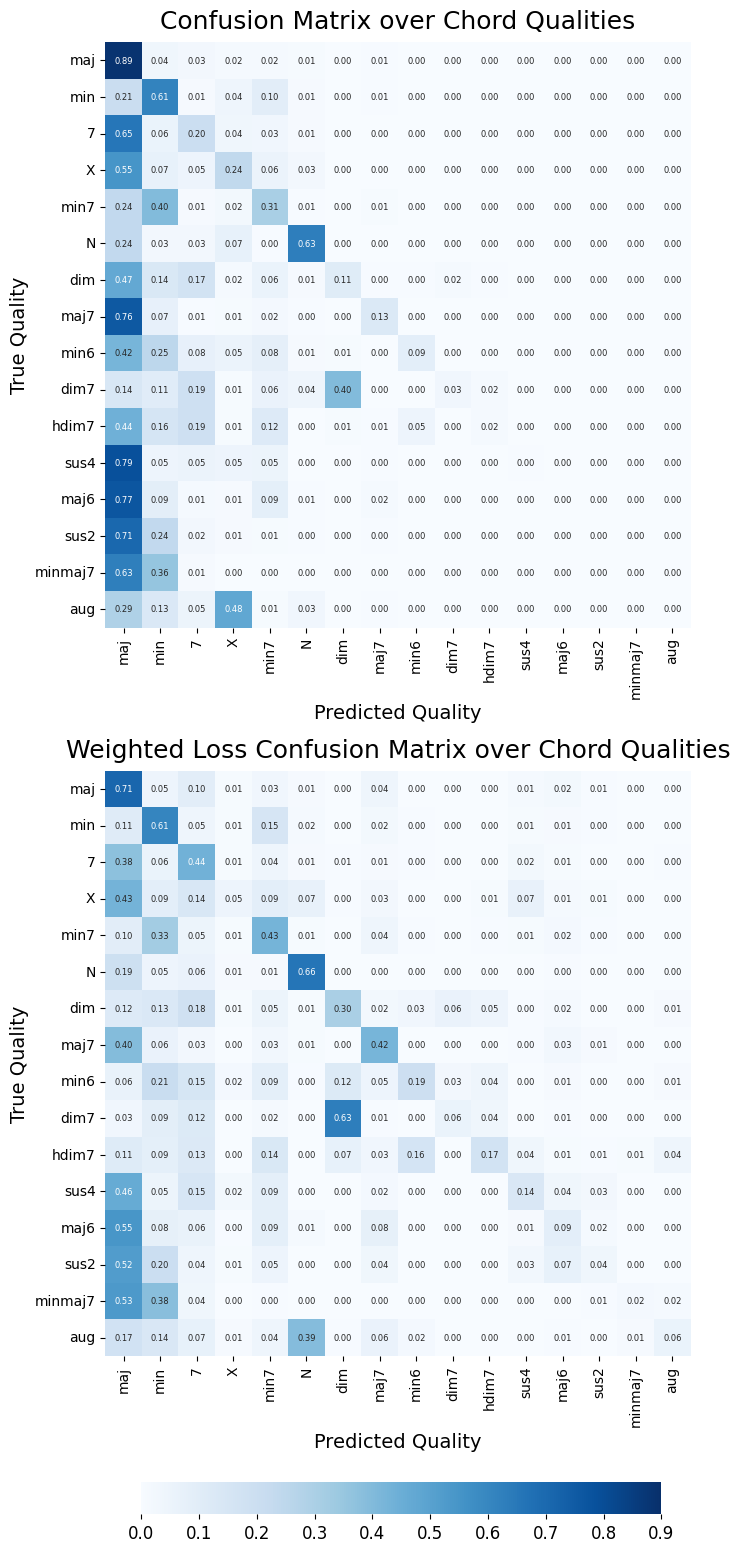
\includegraphics[width=0.68\textwidth]{figures/confusion_matrix_qualities.png}
    \caption{Row-normalised confusion matrices over qualities of the \emph{CRNN} model without (above) and with (below) weighted loss. The weighting is with with $\alpha = 0.55$ as in Equation\ref{eq:weighted_loss}. Rows are ordered by frequency of chord quality. We can see that both models struggle with the long tail. However, weighting the loss does improve the model, notably on \texttt{7} and \texttt{maj7} qualities and predicts \texttt{maj} less often. Recall on the \texttt{maj} worsens by $0.18$ and recall on \texttt{X} decreases from $0.24$ to $0.05$. The weighted model predicts \texttt{X} approximately four times less often. This may be how the weighted model improves class-wise metrics without sacrificing too much overall accuracy, since \texttt{X} frames are ignored. We can also see that both models frequently confuse \texttt{dim7} and \texttt{dim} qualities, consistently predict \texttt{maj} for \texttt{sus2, sus4, maj6, maj7} and \texttt{minmaj7} and struggles with \texttt{aug}.  }\label{fig:crnn_qual_cm}
\end{figure}

\subsubsection{Transition Frames}

We hypothesise that the model is worse at detecting chords on frames where the chord changes. Such transition frames are present because frames are calculated based on hop length irrespective of the tempo and time signature of the song. To test this, we isolate the transition frames and compare the accuracies for transition and non-transition frames separately. We found that with a hop length of 4096, $4.4\%$ of frames are transition frames. On the \emph{CRNN} model with a \texttt{frame} of $0.59$, the model achieves a \texttt{frame} of $0.36$ on the transition frames and $0.60$ on non-transition frames. Therefore, the model is certainly worse at predicting chords on transition frames. However, improving performance on these frames to the level of non-transition frames would only increase the overall frame-wise accuracy by less than $0.01$. 

Through manual investigation explained in Section~\ref{sec:crnn_performance_across_context} we found that on some songs the model did struggle to correctly identify the boundary of a chord change. This was not captured by the above metrics as if the boundary is ambiguous enough to span multiple frames, there may be a larger impact in accuracy than a single frame. Furthermore, some songs will have more obvious boundaries than others. Though the average may be low, for some songs this may be the main limiting factor in performance. However on such songs, the boundaries are likely to be highly subjective and the model would have to learn to detect the beat to consistently predict the boundaries. As previously discussed, we did not wish to introduce another failure mode by using a separate model for beat detection. Some work has attempted to simultaneously segment and predict This is a related task which we do not address here.

Given the above evidence that few frames are affected, and the difficulty of directly addressing the beat detection problem, we do not further investigate transition frames in this work.

\subsubsection{Smoothness}

Are the models outputs \emph{smooth}? Most chords in the dataset last longer than a second but there are more than 10 frames per second. If many of the model's errors are due to rapid hesitation in chord probability, some post-processing smoothness could be applied. We use a crude measure of smoothness by looking at the number and length of incorrect regions. Such a region is defined as a sequence of frames with the same predicted chord where the model predicts the frames incorrectly. We find that of all incorrect regions, $26.9\%$ are one frame wide. However, only $1.7\%$ of frames that are incorrect are one frame wide. Thus, predicting correctly for all one-frame-wide regions would only improve the metrics by $0.017$. A histogram over region lengths can be found in Appendix~\ref{app:histogram_over_region_lengths}.

We conclude that further work on the model to improve the smoothness would not improve performance significantly. However, when being used by a musician, smoothing predictions is valuable to make the chords more interpretable, and perhaps more correct. This is explored as a post-processing step in Section~\ref{sec:decoding}.

\subsubsection{Performance Across the Context}\label{sec:crnn_performance_across_context}

How does the model perform across its context? We hypothesise that the model is worse at predicting chords at the beginning and end of a patch of audio as it has less context on either side. Analysing this will also help to understand if the model is putting its bi-directional context to good use.

To test this, we evaluate the model using the same fixed-length validation conducted during training as described in Section~\ref{sec:training}. We then calculate average frame-wise accuracies over the context and plot them in Figure~\ref{fig:crnn_context}. We use a segment length of $10$ seconds corresponding to $L=108$ frames. We can see performance is worst at the beginning and end of the patch, as expected, but not by much. Performance only dips 5\%, perhaps because the model still does have significant context on one side. We can also see that performance starts decreasing 5 or 6 frames from either end.

We conducted a further experiment, measuring overall accuracy with increasing segment lengths used during evaluation. Indeed accuracy increases, but only by a tiny $0.005$ from 5 seconds to 20 seconds and is flat thereafter. Results can found in Appendix~\ref{app:accuracy_vs_context_length}. We conclude that the context length does not make a big difference and continue to evaluate the model over the entire song at once.

\begin{figure}[H]
    \centering
    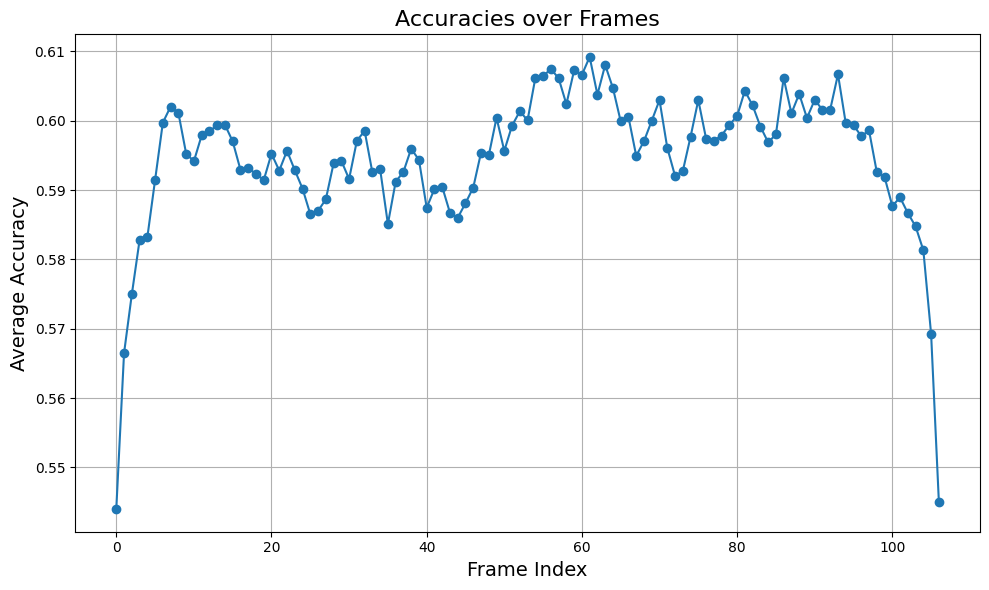
\includegraphics[width=0.8\textwidth]{figures/accuracy_over_frames.png}
    \caption{Average frame-wise accuracy of the \emph{CRNN} model over the patch of audio. The model performs worse at the beginning and end of the patch of audio, as expected. However, the differences are only ~5\%. We propose that the context on one side is enough. This plot supports our procedure of evaluating over the entire song at once. }\label{fig:crnn_context}
\end{figure}

\subsubsection{Generalising Across Songs}

Does the model do well consistently over different songs? We plot a histogram of accuracies and mirex scores over songs in the validation set in Figure~\ref{fig:crnn_song_hist}. We find that the model has very mixed performance with accuracy, with 17\% of songs scoring below $0.4$. However, when we use the more generous \texttt{mirex} metric, almost all of the scores below $0.4$ are improved, and only 6\% below 0.6. Many of the mistakes that the song makes are a good guess in the sense that it may have omitted a seventh or mistaken a major 7 for its relative minor. Examples of such mistakes are discussed in Section~\ref{sec:crnn_examples}. We conclude that, in general, the model's outputs are reasonable predictions, but lacks the detail contained in good annotations like correct upper extensions of the chords.

\begin{figure}[H]
    \centering
    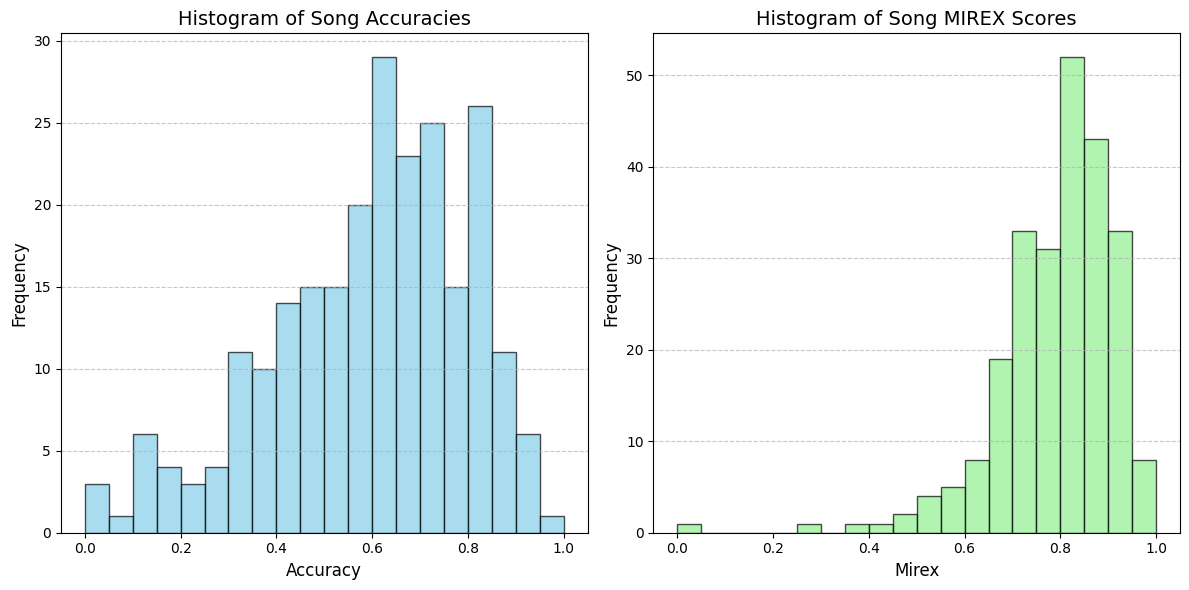
\includegraphics[width=1.0\textwidth]{figures/accuracy_mirex_histograms.png}
    \caption{Histogram of accuracies and mirex scores over songs in the validation set. Accuracies are mixed, with 17\% of songs below $0.4$, and 64\% between $0.4$ and $0.8$. However, with the more generous \texttt{mirex} metric, we find that there are almost no songs below $0.4$ and only 6\% below $0.6$. Many of the mistakes the model makes are small, like predicting \texttt{C:maj} instead of \texttt{C:maj7}. Such examples are discussed in more detail in Section~\ref{sec:crnn_examples}. The very low outliers in the \texttt{mirex} score were found to be songs with incorrect annotations found in Section~\ref{sec:data-integrity}.}\label{fig:crnn_song_hist}
\end{figure}

\subsubsection{Four Illustrative Examples}\label{sec:crnn_examples}

Let us now inspect a few songs to see how the model performs. We choose four examples showing different typical behaviours. We show illustrations of frame-by-frame correctness as measured by both accuracy and \texttt{mirex} in Figure~\ref{fig:crnn_examples}. 

In `Mr.\ Moonlight', there are few differences between the accuracy and mirex. There are regular repeated errors, many of which are mistaking \texttt{F:sus2} for \texttt{F:maj}, which is an understandable mistake to make, especially after hearing the song. As evidenced by the confusion matrices in Figure~\ref{fig:crnn_qual_cm}, this mistake very fairly common on qualities like \texttt{sus2}. In `Ain't not Sunshine', the mirex is significantly higher than the accuracy. This is because the majority of the mistakes the model makes are missing out a seventh. In this song, many of these are a missing seventh such as \texttt{A:min} for the true label of \texttt{A:min7} or \texttt{G:maj} for \texttt{G:7}. Other mistakes that mirex allows for include confusing the relative minor or major, such as \texttt{E:min7} for its relative major \texttt{G:maj}. The mean difference between the accuracy and mirex is $0.2$, with one song reaching a difference of $0.9$. Hence, we can attribute many of the model's mistakes to such behaviour. 

`Ain't no Sunshine' also contains a long incorrect section in the middle. This is a section with only voice and drums which the annotation interprets as \texttt{N} symbols but the model continues to predict harmonic content. The model guesses \texttt{A:min}, which is a sensible label as when this melody is sung in other parts of the song, \texttt{A:min7} is playing. Examples like this combined with incorrect predictions of when a song starts and ends explain the why the mode's recall on the \texttt{N} class is only $0.63$.

In the next two songs, `Brandy' and `Earth, Wind and Fire', the model's mistakes are less interpretable. While performance is okay on `Brandy' with a \texttt{mirex} of $0.74$, the model struggles with the boundaries of chord changes resulting in sporadic short incorrect regions in the figure. In `Earth, Wind and Fire', the model struggles with the boundaries of chord changes, and also often predicts completely wrong chords. This is a song where the model's outputs are less sensible. Listening to the song and inspecting the annotation makes it apparent that this is a difficult song for even a human to annotate well and similarly the model does not fare well.

Despite these mistakes, the average mirex over the validation set is $0.79$ while the accuracy is $0.58$. The examples above highlight the models' errors but the model fares well with many songs. We conclude that the majority of the model's outputs are reasonable predictions but that many lack the detail contained in good annotations like correct upper extensions of the chords. The model confuses qualities that can be easily mistaken for major or minor chords. Sometimes the model makes mistakes in the boundaries of chord changes, and sometimes it predicts completely wrong chords, although these are on songs which are more difficult to annotate.

\begin{figure}[H]
    \centering
    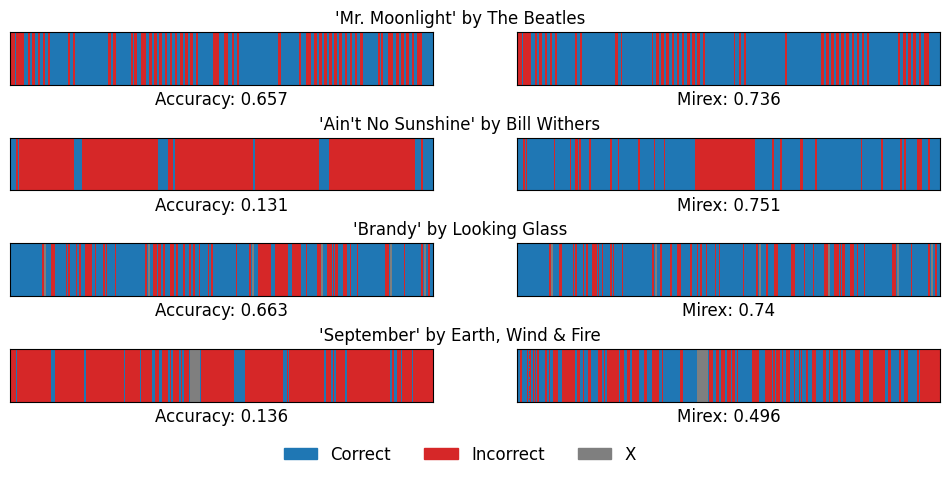
\includegraphics[width=1.0\textwidth]{figures/chord_recognition_examples.png}
    \caption{Chord predictions of the \emph{CRNN} model on four songs from the validation set (blue: correct, red: incorrect, gray: \texttt{X}). This allows to understand some of the behaviour of the model. We can see regular repeated errors in `Mr.\ Moonlight', which are mostly mistaking two similar qualities. The discrepancy between accuracy and \texttt{mirex} on `Ain't No Sunshine' can be explained by missing sevenths in many predictions in `Ain't No Sunshine'. The large incorrect region is a voice and drum only section where the model continues to predict chords due to implied harmony by the melody. Predictions in `Brandy' are quite good in general, though many errors arise from predicting the boundaries of chord changes incorrectly. The model struggles with `Earth,  Wind and Fire', missing chord boundaries, and sometimes predicting completely wrong chords. There are clearly songs where the model's outputs are less sensible. However, in general most of the model's mistakes can be explained and are reasonable.}\label{fig:crnn_examples}
\end{figure}

\section{Weighted Loss}

One of the biggest problems highlighted above is low recall on less common qualities. Two common methods for dealing with long-tailed distributions are re-sampling and weighting the loss function. Sampling is explored by~\citet{BalanceRandomForestACR}. However, they use a different re-weighting scheme based on pre-computing chroma vectors and re-sampling these chroma vectors for use in training a random forest for frame-wise decoding. In our setting, re-sampling training patches of audio may be interesting but is left as future work as it would require significant effort to manage sampling many chords at once. Weighting has been explored by~\citet{ACRLargeVocab1}, and we employ a similar, but simpler implementation here.~\citet{CurriculumLearning} explore the use of curriculum learning as form of re-sampling which we do not explore here.

A standard method of weighting is to multiply the loss function by the inverse of the given class' frequency, with a parameter controlling the strength of the weighting. This is defined as below.

\begin{equation}
    w_c = \frac{1}{(\text{count}(c) + 1)^\alpha}
\end{equation}

Where $w_c$ is the weight for chord $c$, $\text{count}(i)$ is the number of frames with chord $c$ in the dataset and $\alpha$ is a hyperparameter controlling the strength of weighting. $\alpha=0$ results in no weighting and increasing $alpha$ increases the severity of weighting. We add one in the denominator to avoid dividing by $0$. We then define normalised weights $w_c^*$ below.

\begin{equation}\label{eq:weighted_loss}
    w_c^* = \frac{w_c}{s} \text{ where } s = \frac{\sum_{c\in C} \text{count}(c)\cdot w_c}{\sum_{c\in C} \text{count}(c)}
\end{equation}

Where $C$ is the set of all chords in the vocabulary. This keeps the expected weight at $1$ such that the effective learning rate remains the same. We calculate these values over the training set. We test values of $\alpha$ in the set \{0, 0.05, 0.1, \ldots, 0.95, 1\}. The plot in Figure~\ref{fig:weighted_loss} shows the effect of the weighting on the model's performance.

\begin{figure}[H]
    \centering
    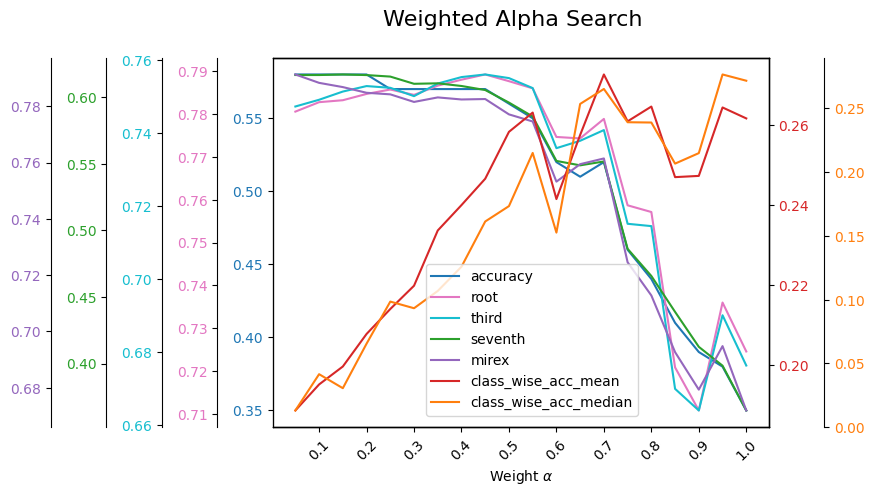
\includegraphics[width=1.0\textwidth]{figures/weight_alpha_search.png}
    \caption{Effect of weighted loss on the \emph{CRNN} model with varying $\alpha$. As we increase $\alpha$, class-wise metrics improve but accuracy-based metrics worsen. We claim a sweet-spot in the middle where we trade only a little overall performance for better class-wise recall. We choose this to be $\alpha = 0.55$. The \texttt{root} and \texttt{third} metrics improve and less than $3\%$ is lost on other metrics while mean class-wise accuracy improves by $6\%$ and the median improved by $0.2$. This plot also reveals strong correlation between metrics. }\label{fig:weighted_loss}
\end{figure}

\section{Pitch Augmentation}
- Two methods:
- On CQT \citet{ACRLargeVocab1}, not good.
- Using MUDA on the audio [everyone else], works?

\section{Structured Training}

- Add structured loss and retrain. From literature. Should (?) further improve accuracies on sevenths etc.

\section{Transformer}

- Make own transformer architecture, similar to BTC or HarmonyTransformer, or Curriculum learning. How to train and evaluate?

\section{Using Generative Features}

- As in [MelodyTranscriptionViaGenerativePreTraining], use Jukebox (?) to generate features at frames (? is it possible to do it on the same frames?). Train on these features and evaluate.

\section{Decoding}\label{sec:decoding}

- HMM
- CRF
- Something ad-hoc?

\section{Results on Test Set}

- Directly compare CRNN, weighted loss, pitch augmentation, structured, transformer, generative features on the test set.